\section{Observing Our Climate}
\label{sec:observing_climate}

As we have seen in previous sections, signals of climate change are quite small
in section \ref{sec:climate-timescales} we see that a 2x in \ce{CO2} concentration
``only'' leads to a few degrees temperature difference. It is of very high 
importance therefore to be able to measure these changes 
\hyperlink{glo:accuracy}{accurately} and \hyperlink{glo:precision}{precisely} 
(see glossary for definitions) as to be able to detect anthropogenic signals
and distinguish them from \textbf{natural variability}.\\

\subsection{Examples of Potential Issues: In-Situ and Ground Based Measurements}
\label{sec:issues}

\subsubsection{The Urban Heat Island Effect}
\label{sec:uhi}

\begin{figure}[h]
    \centering
    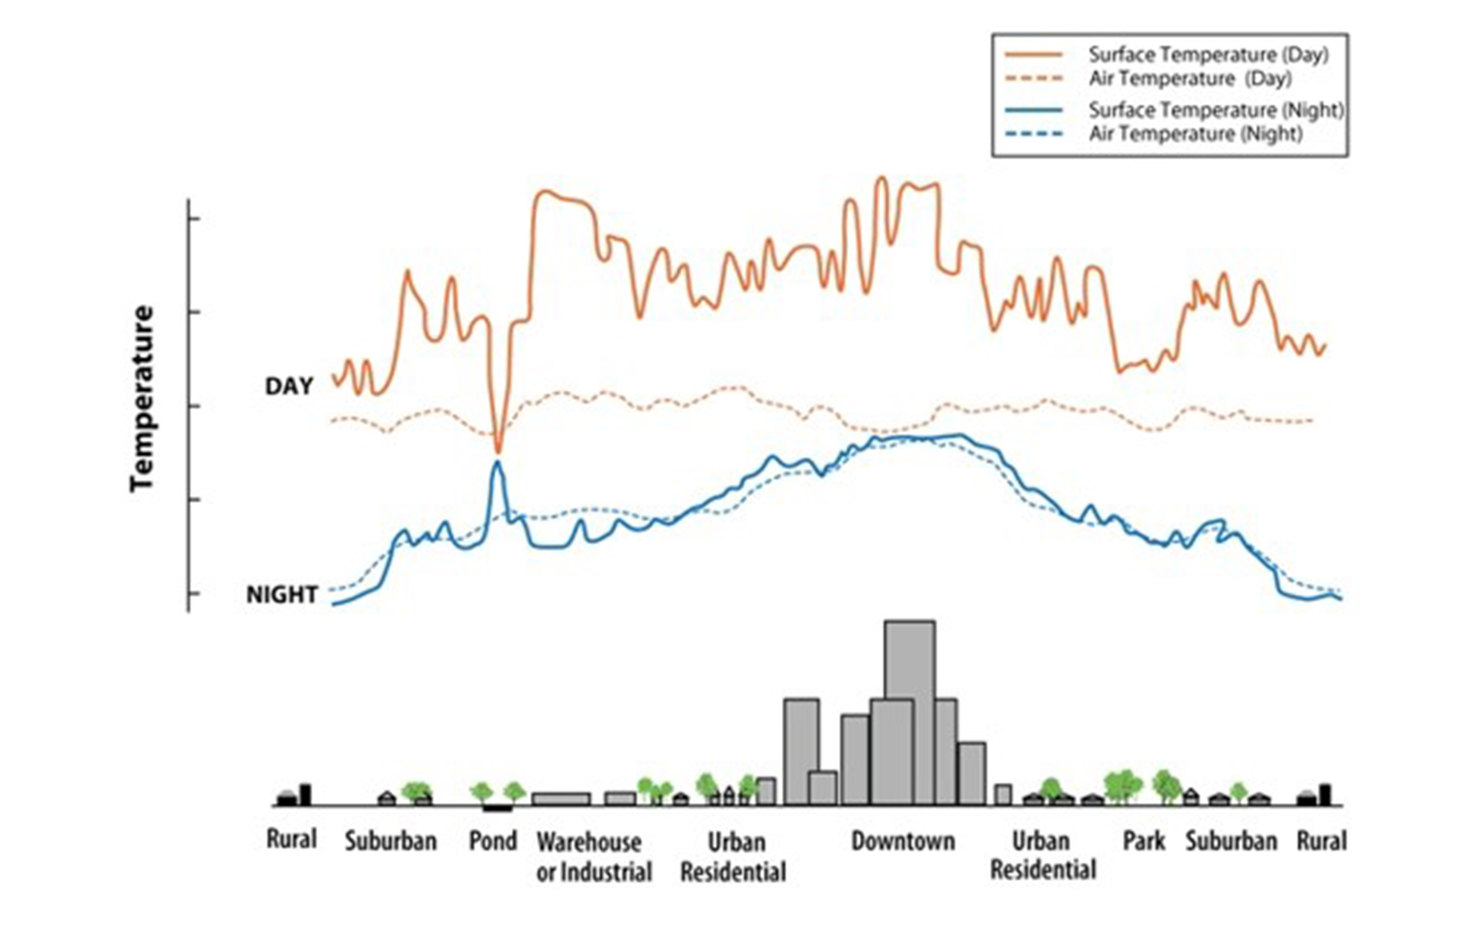
\includegraphics[width=0.65\textwidth]{figures/urban_heat_island.jpeg}
    \caption{Urban Heat Island Effect.}
    \label{fig:uhi}
\end{figure}

Figure \ref{fig:uhi} shows a schematic of the \textbf{urban heat island effect}.
This is a phenomenon where urban areas are warmer than their rural surroundings.
This is especially true at night. Some reasons for this are:
\begin{itemize}
    \item \textbf{Albedo}: Urban areas have a lower albedo than rural areas. 
    This means that they absorb more \gls{SW} radiation and therefore heat up 
    more. This is obvious when we consider that some key urban materials like 
    asphalt have an albedo much lower of that of vegetation.
    \item \textbf{Thermal Inertia}: Urban areas have a lower thermal inertia than
    rural areas. This means that they heat up more quickly during the day and cool
    down more quickly during the night. The fact that they heat up more during
    the day means that they release more heat during the night, further Increasing
    temperatures at when the sun does not shine.
    \item \textbf{Anthropogenic Heat}: Urban areas have a higher concentration of
    anthropogenic heat sources (cars, air conditioning, heating, etc.) than rural areas.
    \item \textbf{Evapotranspiration}: Urban areas have a lower evapotranspiration
    rate than rural areas. This means that less energy is used to evaporate water
    and more energy is used to heat the air. This is the case due to the lack of
    vegetation and bodies of water (ponds, lakes, etc.) in urban areas.
\end{itemize}

We can define the \textbf{Urban Heat Island Index} (somehow abbreviated UHI) as
the maximum temperature difference between the urban and rural areas as a function
of time:
$$
\boxed{
\text{UHI}(t) = \max(T_{\text{urban}}(t) - T_{\text{rural}}(t))
}
$$
which as previously mentioned is usually larger at night. In fact during the day
it is only usually the air that is closest to the ground that is different. We 
can also consider the following \textbf{surface energy balance}:
$$
(R_S^{\downarrow} - R_S^{\uparrow}) + (R_L^{\downarrow} - R_L^{\uparrow}) = H + E + Q
$$
where the $R_S$ terms represent the net downward \gls{SW} radiation at the surface,
the $R_L$ terms represent the net downward \gls{LW} radiation at the surface, $H$
is the sensible heat flux\footnote{Sensible heat flux means that is heat that can be ``sensed'',
or measured, usually with a thermometer. Latent heat flux in contrast cannot be
measured with a thermometer.}, $E$ is the latent heat flux and $Q$ is the ground heat 
transfer. It therefore follows that each of right hand side terms are affected 
due to urban characteristics.\\

It is therefore obvious that having measurement stations in/near urban areas will
lead to a bias in the measurements. This is a problem because most of the
\textbf{long term climate records} are based on measurements from urban areas.
Without corrections, warming trends would be amplified due to urbanisation.

\subsubsection{Changes in Sensor Design/Instrument Characteristics}
\label{sec:changes_in_sensor_design}

A clear example of how changes in how measurements are taken can lead to biases
in the data is the change in the design of \textbf{sea surface temperature} 
(\gls{SST}) measurements. There are a number of ways in which \gls{SST} measurements
can be taken including floating buoys, bucket measurements, hull contact sensors
and ship engine intake. It is clear, especially for the latter two measurement
methods, that the readings will have a bias. Such biased measurement techniques
are being phased out as we move towards more accurate and precise methods so 
once again it is crucial to make corrections when comparing new and old data.
See L9 for lower-level details.\\

Another example of this is the change in the design of global \textbf{radiosonde}
network. Radiosondes are instruments that are attached to weather balloons and
measure atmospheric parameters (temperature and humidity) as they ascend through
the atmosphere. The first measurements date back to the early 1900s so it is 
clear that the design of the instruments has changed significantly since then.
Furthermore, different regions of the world have used different typer of sensors
so once more it is crucial to make corrections when comparing new and old data 
and when comparing data from different regions when making a globally homogeneous
record.

Examples of what can cause discrepancies across different sensors include:
\begin{itemize}
    \item \textbf{Time constant}: The time it takes for the sensor to reach a new
    temperature after a change in temperature. This arises due to the sensor's
    \gls{thermal_inertia}.
    \item \textbf{Material composition}: Different materials have different
    \gls{emissivity} and \gls{absorptivity} characteristics, meaning that they
    will absorb and emit different amounts of radiation.
    \item \textbf{Sensor location}: The length of the string attaching the sensor
    to the balloon can affect the readings. This is because the balloons tend to
    have warmer temperatures than the environment around them.
\end{itemize}

\subsection{Surface Temperature Trends and the Impact of Satellite Observations}
\label{sec:surface_temp_trends}

Despite the issues mentioned above, after applying the necessary corrections,
we can still se a warming trend of about 1K over the last 100 years and this 
warming is more accentuated over land than over the oceans as per section 
\ref{sec:climate-timescales}.\\

Satellite observations have become a standard practice since the late 1970s for 
gathering data on the state of the atmosphere and surface, including 
temperature and humidity. These observations offer significant advancements over
traditional surface and in-situ measurements, evident in their higher spatial 
resolution and the availability of a more comprehensive and global sea-surface 
temperature (\gls{SST}) record starting from the late 1970s.

\subsection{Space-Based Observations}
\label{sec:space_based_obs}

In the previous section we outline some of the advantages of space-based
observations when compared to ``legacy'' means of climate observation. However,
space-based observations come with challenges and limitations of their own.\\

\noindent There are two main types of space-based sensors:
\begin{itemize}
    \item \textbf{Passive Sensors}: These sensors measure the \gls{LW} 
    radiation emitted by the Earth and backscattered light from the Sun. These
    are the most common type of sensors and have been used since the beginning
    of the space-based observation era to measure surface and atmospheric
    temperature.\\
    These are low-power devices so they are able to scan large portions of the
    Earth.
    \item \textbf{Active Sensors}: These newer sensors emit their own radiation and
    measure the amount of radiation that is reflected back to them (LIDAR, RADAR).
    These kind of sensors are particularly good at measuring clouds and aerosols
    and their vertical structure.\\
    These are high-power devices so they are only able to scan small portions of
    the Earth at once.
\end{itemize}

\noindent The climate variable that a sensor is measuring will be dependent on 
the wavelength examined by it. Always remember that the only kind of interaction
between the Earth and a satellite will be through \textbf{photon exchange}.

Up to now we have mostly considered \textbf{irradiance} $I_\lambda$: the amount
of energy per unit area per unit wavelength emitted or recieved from all directions
such that at the \gls{TOA} we have:
$$
\text{\gls{OLR}} = \int I_\lambda \text{d}\lambda
$$
but most satellite sensors measure \textbf{radiance} $L_\lambda$: the amount of
energy per unit area per unit wavelength per unit solid angle recieved from a
particular direction. Newer satellites are able to measure radiance in multiple
directions. Furthermore, it follows that if we are interested in these instruments
giving us insight into the temperature of the surface or the atmosphere that 
the light captured by these must be in the \gls{LW} part of the spectrum.

\begin{tcolorbox}
    \textbf{Aside on Radiance vs Irradiance}:\\

    Let's consider an observational instrument in space aimed at Earth, designed
    to measure Earth's reflected and emitted energy.\\

    \noindent \textbf{Irradiance}:

    Suppose the instrument is equipped with a sensor that measures the total 
    power incident on it per unit area from Earth, integrating over the entire
    field of view. This sensor does not differentiate between the various regions
    on Earth's surface it's viewing - it's simply recording the total power from
    all these regions per unit area. The measured quantity is the irradiance at 
    the sensor's location, arising from the totality of the Earth scene within 
    its field of view.\\

    \noindent \textbf{Radiance}:

    Now, consider a different instrument on the same platform, but this one is a
    hyperspectral imaging device - a bit like a camera sensor that can capture
    many different wavelengths and has many pixels. 
    This instrument is designed to measure the
    power received in each of its pixels per unit area per unit solid angle. 
    Each pixel corresponds to a specific area on Earth's surface, and the 
    instrument measures the power coming from that specific area and direction. 
    For each pixel, it quantifies the power received in each of a multitude of 
    narrow spectral bands, thereby providing a spectrum for each pixel.\\

    The quantity it measures is radiance. It is a directional quantity, 
    associated with a specific location (the corresponding surface area) and a 
    specific direction (the direction from that area to the instrument). \\

    For a given location on Earth's surface, the radiance varies with the direction.
    For example, if the location is a forest, the radiance in the direction of the 
    sun may be quite different from the radiance in a direction away from the sun, 
    due to the scattering properties of the trees. \\

    Therefore, while irradiance gives a measure of the total power per unit area
    received from all directions, radiance provides a detailed picture of the 
    power per unit area received from each specific direction. This allows for
    a more nuanced understanding of how light interacts with Earth's surface 
    and atmosphere.
\end{tcolorbox}


\subsection{Obtaining Temperature Information from Space and Schwarzschild's 
Equation}
\label{sec:schwarzschild}

To obtain temperature information from space we need to consider the following:
\begin{itemize}
    \item The interaction between the Earth's emmited \gls{LW} radiation and the
    atmosphere.
    \item How to describe these interactions mathematically.
    \item Translate this to temperature measurements from space.
\end{itemize}

\subsubsection{Interaction Between LW Radiation and the Atmosphere}
\label{sec:lw_atm}

There are three main ways in which \gls{LW} radiation interacts with the 
atmosphere: \textbf{absorption}, \textbf{emission} and 
\cancel{\textbf{scattering}}. We can neglect scattering in the \gls{LW} in times
of clear-sky conditions. This is not the case if there are clouds, but in such a
case we cannot measure the surface temperature anyway.\\

We can begin by considering absorption by a layer of atmosphere $dz$. As per the
\gls{beer_lambert}, we have the following:
$$
dL_{\lambda \text{abs}} = -L_\lambda \rho_{\text{a}} \kappa_\lambda^{\text{a}} dz
$$
where $dL_{\lambda \text{abs}}$ is the change in radiance due to absorption,
$L_\lambda$ is the incident radiance at the base, $\rho_{\text{a}}$ is the density
of the absorbing material and $\kappa_\lambda^{\text{a}}$ is the mass absorption 
coefficient.\\

Secondly, we consider the emission by a similar layer of atmosphere $dz$. As per
\gls{kirchoff} (\gls{LTE})we have the following:
$$
dL_{\lambda \text{em}} = B_\lambda(T_z) \rho_{\text{a}} \kappa_\lambda^{\text{a}} dz
$$
where $dL_{\lambda \text{em}}$ is the radience emmited by the layer, $B_\lambda(T_z)$
is the \textbf{Plank Function} at the temperature of the layer $T_z$ and
$\rho_{\text{a}} \kappa_\lambda^{\text{a}}$ is the \gls{emissivity} (equal to the
\gls{absorptivity}).

We can combine these two equations to obtain the following:
$$
dL_{\lambda} = -[L_\lambda + B_\lambda(T_z)] \rho_{\text{a}} 
\kappa_\lambda^{\text{a}} dz
$$
and bring in the concept of \hyperlink{glo:opticaldepth}{optical depth} 
$\tau_\lambda$ do do the following derivation:
\begin{gather*}
    \tau_\lambda = \int \rho_{\text{a}} \kappa_\lambda^{\text{a}} dz \quad 
    \implies \quad d\tau_\lambda = \rho_{\text{a}} \kappa_\lambda^{\text{a}} dz\\
    dL_{\lambda} = -[L_\lambda - B_\lambda(T_z)] \rho_{\text{a}} 
    \kappa_\lambda^{\text{a}} dz\\
    \frac{dL_{\lambda}}{d\tau_\lambda} + L_\lambda = B_\lambda(T_z)\\
\end{gather*}
which is a first order ODE that we can solve for $L_\lambda$ using an 
integrating factor and the following boundary conditions (see L10 for more 
details):
$$
\boxed{
\textcolor{orange}{L_\lambda(z_{\text{space}})} = 
\textcolor{blue}{L_\lambda(0)e^{-\tau_\lambda}} + 
\textcolor{red}{\int_0^{\tau_\lambda}B_\lambda(T_z) 
e^{-(\tau_\lambda - \tau_\lambda')} d\tau_\lambda'}}
$$

This is the \textbf{Schwarzschild Equation}. The term in \textcolor{orange}{orange}
is the radiance seen by the satellite, the term in \textcolor{blue}{blue} is the
radiance emitted by the surface that reaches the satellite despite the absorption
by the atmosphere and the term in \textcolor{red}{red} is the radiance emitted
by the atmosphere that reaches the satellite.

We can rewrite the above equation in terms of \textbf{\gls{transmissivity}} where
we use the following notation to write transmissivity of the atmosphere from 0
to $z_{\text{space}}$: $t_\lambda (0, z_{\text{space}}) = e^{-\tau_\lambda}$:
\begin{gather*}
    t_\lambda(z', z_{\text{space}}) = e^{-(\tau_\lambda - \tau_\lambda')} \quad
    \implies \quad \frac{dt_\lambda(z', z_{\text{space}})}{d\tau_\lambda'} =
    e^{-(\tau_\lambda - \tau_\lambda')}\\
\end{gather*}
and we obtain the Schwarzschild Equation in terms of transmissivity:
$$
\boxed{
    L_\lambda(z_{\text{space}}) = L_\lambda(0) t_\lambda(0, z_{\text{space}}) +
    \int_{t_\lambda(0, z_{\text{space}})}^1 B_\lambda(T_z) 
    dt_\lambda' (z', z_{\text{space}})
}
$$

Remember that we make the assumption that \textbf{the atmosphere is in \gls{LTE}}
and that there is \textbf{no scattering}.

\subsubsection{Weighting Functions}
\label{sec:weighting_functions}

When we attempt to retrieve temperature information from space, we will not use
the Schwarzschild Equation as written above, but rather we transform it into the
following in terms of altitude $z$:
$$
\boxed{
    L_\lambda(z_{\text{space}}) = L_\lambda(0) t_\lambda(0, z_{\text{space}}) +
    \int_{z=0}^{z_{\text{space}}} B_\lambda(T_z) \textcolor{red}{
    \frac{dt_\lambda' (z', z_{\text{space}})}{dz}} dz
}
$$
where the term in \textcolor{red}{red} is the \textbf{weighting function} 
$K_\lambda(z)$. Note that the weighting function could be defined in terms of 
any other variable so long as it is monotonic\footnote{Monotonic means that one
variable is either always increasing or always decreasing with respect to the
other variable. It also ensures that there is a one-to-one correspondence between 
variables. E.g. pressure and height.} with height.

The concept of a weighting function is a useful one because it allows us to
understand where from the atmosphere a particular wavelength is coming from as
measured by a satellite.

It follows that by scanning a number of different wavelengths we are able to 
obtain a vertical profile of the atmosphere for the particular feature we are 
interested in\footnote{This requires a constant gas density, so usually the \ce{CO2}
band is used} e.g. temperature, humidity, etc. Finally then, the higher the 
spectral resolution (i.e. the narrower the range of wavelengths the satellite
measures) the more vertical information the satellite can obtain.

\subsection{Issues With Satellite Based Records}
\label{sec:issues_satellite}

As with any other kind of measurement, satellite based measurements are not
without their own issues. Some of these include:
\begin{itemize}
    \item \textbf{Accuracy of Calibration}: Instruments must be callibrated 
    against a known reference or standard prior to launch to space as to convert
    a measurement to the required quantity. The \textbf{transfer of callibration}
    from ground to space is often unstable.
    \item \textbf{Length of Missions and Consistency of Instrumentation}: A 
    typical mission will last for about 3-5 years. This means that instruments 
    are replaced somewhat regularly, and although they are replaced with newer 
    and potentially slightly different equipment as to exploit new technologies,
    which can lead to inconsistencies in the data.
    \item \textbf{Orbit Decay}: The orbit of a satellite will decay over time
    due to atmospheric drag. This means that the satellite's altitude changes
    leading to changes in the measured signal.
    \item \textbf{Gaps in Data}: If launches are delayed, or if the satellite
    in orbit malfunctions and there are no others that can take over, then there
    will be gaps in the data.
    \item \textbf{Inversions}: Inversions are the process of transforming 
    satellite measurements into the required quantity. Like we have seen above,
    these inversions are ``models'' and as such have their limitations and 
    assumptions. It therefore follows that different models will yield different
    insight with the same data. (There is some extra detail in the last few 
    slides of L10, mainly examples).    
\end{itemize}

